
Methodology comes first (\S{}3.1), then the problem and its constraints (\S{}3.2), then the design and the seven predicate rules following from it (\S{}3.3--\S{}3.11), with the legal and ethical constraints in \S{}3.12 and every decision collected in one table in \S{}3.13.

\section{Research methodology}

Three process models dominate data-science practice. \textbf{KDD} (Fayyad, Piatetsky-Shapiro and Smyth, 1996) treats the work as a nine-step pipeline for finding patterns in existing databases. \textbf{SEMMA} compresses that into five tool-centred stages. \textbf{CRISP-DM} (Wirth and Hipp, 2000) adds what both lack, which is an explicit \textit{Business Understanding} phase before any data is touched, together with a cycle in which evaluation feeds back into the earlier phases. Azevedo and Santos (2008) find it is effectively a superset of SEMMA, with stronger process guidance than KDD.

Two reasons decided it. Since the motivating problem is an engineering question posed by a dataset's own authors, a phase pinning that problem down before any modelling is necessary, not decorative. The project also ran the way CRISP-DM's evaluation-to-modelling loop describes and the linear models do not, since the audit of support-rule precision sent me back to modelling twice, for a depth gate and then a mask-contact test, each re-validated on held-out annotators. Section 1.3 maps every phase to a part of this dissertation, including the two findings from Data Understanding, and summarises the ethical considerations detailed in Supplementary A.

\section{Problem analysis}

From a raw robot-acquired RGB image the pipeline has to produce what a human annotator does with SGDET-Annotate: a scene graph over the six object classes with the seven spatial predicates, exported in Visual Genome JSON, YOLO txt and h5. Four requirements shape the design:

\begin{enumerate}
\item \textbf{No human decides any label.} A rule may abstain and flag, but it may not
ask. 2. \textbf{Comparability with the human labels.} RQ1 needs the outputs to line up with the human annotations pair-for-pair and byte-for-byte in format, or no fair comparison is possible. 3. \textbf{Modest hardware.} A single 6 GB RTX 2060, so anything heavier has to be optional. (In practice the pipeline peaks at 0.65 GB and annotates the full dataset in about five minutes \textit{(measured)}.) 4. \textbf{Reproducibility.} Every threshold in one config, every run seeded, and rule changes re-evaluable without re-running perception.
\end{enumerate}

Three properties of the dataset, established in Chapter 2 and checked on the released files, force the design's hand. Each one forces a design response:

\begin{itemize}
\item \textbf{Monocular RGB only.} There is no metric depth, and estimated depth is \textit{relative and per-image} (Yang, L. et al., 2024). So every depth comparison is ordinal and within-image, and no rule consumes absolute depth.
\item \textbf{Sparse annotation.} Humans labelled a minority of object pairs \textit{(measured: 6,458 of 42,440 unordered pairs, 15\%; 8,790 of 84,880 ordered, 10\%, the two differing because most labelled pairs carry only one direction, \S{}4.5)}. The tool labels every pair instead, since density is what it adds, and the protocol treats human labels as a recall target rather than an exhaustive gold standard.
\item \textbf{Inconsistent \texttt{near}.} Three of the nine annotator groups supplied 714 of the 717 \texttt{near} labels (461/160/93). A fourth supplied three and five supplied none. Each labelled a different fraction of equally-close pairs, so the threshold is fitted and annotator-aware (\S{}3.8). There is no consensus to match it to.
\end{itemize}

\section{Design principle: compute, don't predict}

Learned scene-graph generators (REACT++ and predecessors; Neau and Falomir, 2026) \textit{predict} relations from visual patterns, so they need labelled training data and sit downstream of annotation. This pipeline \textit{computes} relations from measured geometry with deterministic rules, so it runs before any learned model and supplies what they consume, which works only because the seven predicates are spatial, each decidable from positions, extents and depth order. There is one exception, which the design concedes and does not hide. Support turns on whether a thing is resting or being held, which geometry cannot represent, so a class guard stands in (\S{}3.6) and ablation A10 finds geometry cannot take that job back (Supplementary D.8), leaving the principle outright for six predicates and for support only up to one semantic list. SAM2 and Depth Anything only \textit{measure} where things are. No learned component decides a relationship. Another route was to keep the human labels and stretch them, with semi-supervised pseudo-labelling or active learning. Section 2.4 sets out that rival and the three properties of this dataset arguing against it, and \S{}5.3 runs the self-training loop as a third arm of the same experiment, so the two routes meet on the humans' own held-out annotations, not on plausibility.

\textbf{Evaluation setting.} Evaluation of the relation stage uses ground-truth boxes and classes (\textit{PredCls}, \S{}2.7). That isolates the contribution, since the paper already establishes detection at 0.93 mAP@50 with YOLOv10m, and it lines object indices up one-to-one with the human records, while detector-in-the-loop operation stays available as an ablation and as the deployment mode for new images.

\section{Pipeline architecture}

\begingroup\small\begin{verbatim}
image -- boxes+classes --> SAM2 masks --> depth map --> per-object geometry
                                                            |
        writers (VG JSON / YOLO / h5) <-- flags <-- correction <-- 7 rules
\end{verbatim}\endgroup

\needspace{31.2\baselineskip}
\begin{center}
\setlength{\tabcolsep}{3pt}
\footnotesize
\begin{longtable}{>{\raggedright\arraybackslash}p{0.121\textwidth}>{\raggedright\arraybackslash}p{0.292\textwidth}>{\raggedright\arraybackslash}p{0.188\textwidth}>{\raggedright\arraybackslash}p{0.336\textwidth}}
\caption[Pipeline stages, the alternative rejected at each stage]{Pipeline stages, the alternative rejected at each stage, and the justification.}\\
\hline
Stage & Choice & Rejected alternative & Justification \\
\hline
\endfirsthead
\hline
Stage & Choice & Rejected alternative & Justification \\
\hline
\endhead
Boxes & ground truth (study); YOLOv10m / Grounding DINO (deployment) & detector inside RQ1 & isolate the relation stage (\S{}3.3) \\
Masks & SAM2 (Ravi et al., 2024), box-prompted, \texttt{sam2.1-hiera-small}; multimask + best score & boxes only & mask centroids and masked depth are robust to box slack; single-mask mode returned empty masks on loose boxes \textit{(measured)}; box-only kept as an ablation \\
Depth & Depth Anything v2 \textbf{Small} (Yang, L. et al., 2024), HF pipeline & Base/Large; stereo/metric methods & 6 GB budget; Apache-2.0 (Base/Large are non-commercial); no metric depth exists for this data \\
Lift & centroid (x, y) + \textbf{median} depth over the mask & mean depth; full 3D reconstruction & median resists edge bleed where masks overlap background; reconstruction is unnecessary for ordinal tests \\
Fallback & empty mask $\rightarrow$ box region & image centre / drop object & a failed segmentation must not move the object; regression-tested \\
Rules & explicit thresholds, one function per predicate & learned relation head & the graded contribution; auditable and fittable \\
Correction & reject impossible label sets, demote to flags & emit everything & geometric consistency is checkable for free; adapted from Open3D-VQA's correction flow (Zhang et al., 2025) \\
Confidence & flag ambiguity bands for optional review & silent guesses & human-in-the-loop accelerator claim needs an explicit abstention mechanism \\
Writers & byte-compatible VG JSON / YOLO / h5 & own schema + converter & drop-in comparability (requirement 2); verified against real exports \\
\hline
\end{longtable}
\end{center}

Coordinates are normalised, depth is inverted and normalised per image, and an EXIF-aware loader makes the 180$^{\circ}$-rotated captures upright before anything is read. Supplementary C.11 gives all three, along with the sign error that held front/behind agreement at \textasciitilde{}26\% until it was found, against \textasciitilde{}74\% after.

\section{The seven rules}

Supplementary C carries the complete specification, every rule, threshold and shipped value with its evidence, along with the correction and flagging policy, and I keep it in the repository as \texttt{docs/predicate\_\allowbreak{}spec.md}, the copy the code and tests are checked against. The rationale in one pass:

\textbf{on / under} encode \textit{support}, meaning the subject is above the object, near-touching, with horizontal extents overlapping. That last condition stops "floating in front of" reading as "on". \texttt{under} is the strict inverse, so the pair can never contradict. \textbf{to the left of / to the right of} compare horizontal centres in the camera frame, the frame the annotators saw on screen and the faithful choice among RoboSpatial's three (Song et al., 2025), with an ambiguity band that abstains when the centres nearly coincide. \textbf{in front of / behind} is a two-stage cascade. Depth ordering decides first, with an abstention band. These are the hardest predicates, because objects on the same surface often differ by less than the depth model can resolve, and where depth abstains a \textbf{ground-plane fallback} decides from projection, ordering two objects on one floor by which box bottom sits lower. That gives a pixel-precise cue where depth is noisiest, guarded by the tool's own support evidence so it never fires when either object rests on another, while pairs both stages abstain on are flagged and never guessed (recall 0.70/0.71 \textit{(measured)}, up from 0.52/0.55 depth-only). \textbf{near} is a size-relative proximity test, taking the edge-to-edge box gap over mean object size, below a fitted threshold, and \textbf{never on contact pairs}, since \texttt{near} co-occurs with on/under on 0 of 469 human pairs. Figure~\ref{fig:near-T-sweep} shows the sweep the threshold is read off. I rejected a 3D-centroid metric on the evidence, every centroid variant transferring to held-out annotators at F1 $\leq$ 0.024 against the relative gap's recall 1.0 (\S{}3.8).
\begin{figure}[!htbp]
\centering
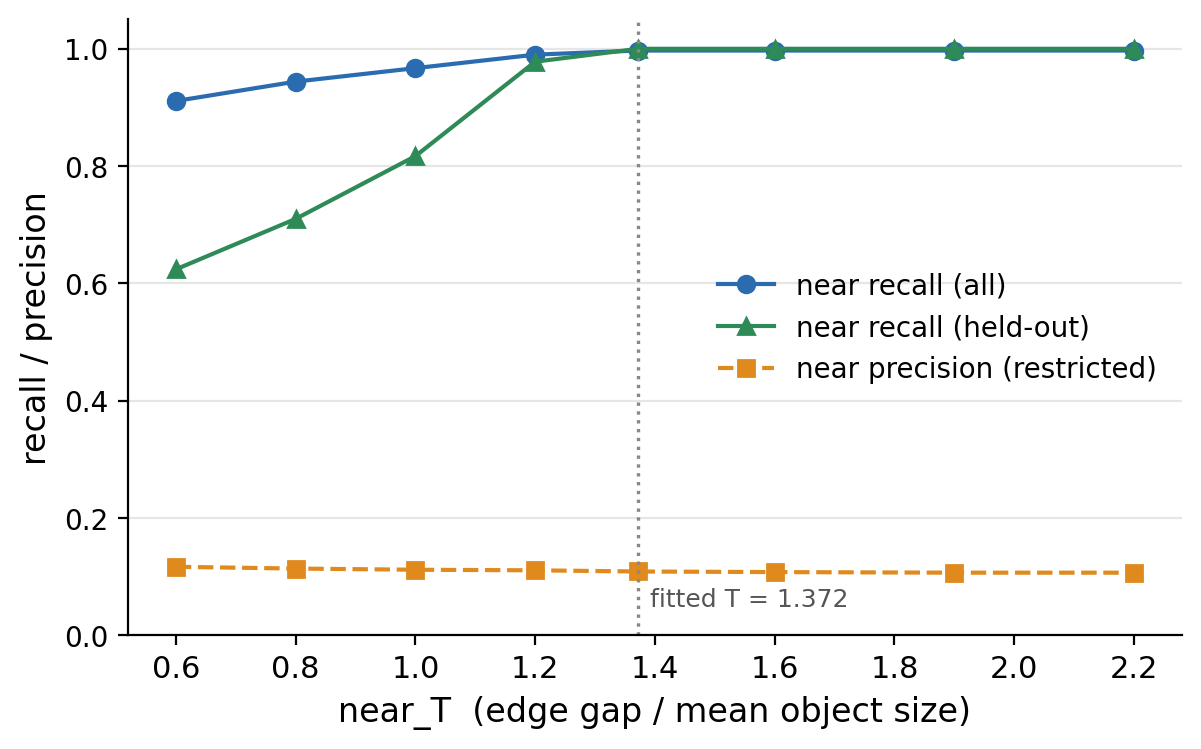
\includegraphics[width=0.80\textwidth,height=0.78\textheight,keepaspectratio]{figures/near-T-sweep.png}
\caption[Fitting the near threshold]{Fitting the \texttt{near} threshold. Recall against all annotators and against the held-out annotator, with restricted precision. The fitted value is the tightest threshold at the plateau.}
\label{fig:near-T-sweep}
\end{figure}


\section{Correction and confidence}

Each of the predicate families, on/under, left/right and front/behind, is mutually exclusive. Two cannot contradict, because the rule branches. Support differs, because \texttt{on} and \texttt{under} are independent tests over \textit{different} contact evidence, so noise in either can make both fire on one pair, and that case is demoted to an \texttt{on\_\allowbreak{}under\_\allowbreak{}conflict} flag with neither label emitted. The tool demotes and does not resolve, because an annotator that fabricates under uncertainty cannot be audited. One further correction is class-aware, not geometric, since support is never evaluated when either object is a person, the annotators having recorded one on \textbf{0 of 2,466 gold support triplets}, and ablation A10 finds geometry cannot replace it (Supplementary D.8). Supplementary C.11 gives both arguments in full. Four kinds of ambiguity flag travel with the triplets, lateral tie, depth tie, near-threshold edge, and the resolved contradiction above. I offer the tool as a human-in-the-loop accelerator with a \textit{measurable} residual cost, not as an oracle, so it has to say when it does not know. About a third of ordered pairs carry a flag, which \S{}4.7 splits into silent abstention and a much smaller review queue. The structural guarantees this section promises are asserted in a randomised invariant test over two thousand synthetic scenes (\S{}3.11), because they hold by construction and a later rule edit could otherwise break them quietly.

\section{Output compatibility}

Byte-compatibility belongs to the research design, and is not a convenience. RQ2 compares two label sources by training the same model on each, so different containers would confuse the labels with the loader. Three consumers are covered by the writers. Visual Genome JSON is what a replication would diff against, YOLO txt trains the detector that the deployment mode and the benchmark share, and the h5 layout is what Chapter 6's framework ingests. Each reproduces the SGDET-Annotate structure exactly. The alternative, an internal schema plus a converter (\S{}3.4), would have put a translation step between every comparison and what it claims to measure, while Supplementary B lists the fields and the round-trip tests that verify them, so auto-labels are drop-in replacements for human ones, which RQ2 depends on.

\section{Calibrating \texttt{near}: an annotator-aware protocol}

Fitting one threshold to all \texttt{near} labels and testing on held-out images fails outright, and held-out F1 comes out at 0.009, because only three of nine groups applied the label in quantity, with very different exhaustiveness. So the protocol fits on human-\textit{annotated}, non-contact pairs from the training-split groups that used the label at all, and reports agreement on the held-out near-user who contributed nothing to the fit. Supplementary C.11 gives the reasoning behind each of those three choices. The results \textit{(measured)}: fitted \textbf{T = 1.372} in gap/mean-size units, and held-out recall \textbf{1.000}, every pair the unseen annotator called near lying inside the threshold. Recall is 1.0 for all three near-using annotators at once, so their labels point the same way as a single threshold. What varies between them, by about fourfold, is how exhaustively each applied it. A fitted threshold applies one definition uniformly, exactly the "spatial thresholds for near" the source paper's future work asks for. Whether the tool's extra near pairs are genuinely near is a separate question, checked by manual audit in Chapter 4.

\section{Modularity: the detector as the replaceable part}

Whether the rules are really detector-agnostic (\S{}4.11) rests on the architecture. My rule layer (\texttt{src/predicates.py}) imports nothing but \texttt{numpy} and never receives an image, and since the entry point takes boxes as an argument, no detector is wired in. You just supply that argument. That is what makes \S{}4.11's conditional measurement meaningful, since fixed boxes let detector and relation quality be attributed separately, and a better detector improves the system without a line of rule code changing. Supplementary B gives the contract, its three implementations, the twelve tests that pin it, and the two documented coupling points. One of those is that a detector drawing systematically different boxes should re-run \S{}3.8's calibration.

\section{Selecting frames by content}

Being consecutive frames of a continuous robot capture, the images oversample the scene badly, as the numbers make plain. Across its 2,650 frames the mean optical flow between neighbours is 0.08 px, so a per-frame pipeline spends a full perception pass on relations that have not moved. What is wanted instead is one frame per \textit{viewpoint}.

Shot-boundary detection will not supply it, because thresholding consecutive-frame differences assumes cuts to find, and 0.08 px never exceeds the noise at a single step, even though the same motion over forty frames displaces the image by 13 px. Only accumulated drift carries the signal. So \texttt{segment\_\allowbreak{}sequence} (\texttt{src/keyframes.py}) measures drift from the \textit{anchor} of the current segment rather than from the preceding frame, so gradual motion accumulates, a genuine cut still crosses in one step, and each segment nominates the frame closest to its mean signature. One parameter covers two uses, since a small $\tau$ isolates near-duplicates while a large $\tau$ groups viewpoints of one arrangement, what \S{}4.12's measurement consumes. Supplementary E.2 gives the thumbnail distance, the sweep, and what the segmentation recovers.

\section{Reproducibility by construction}

Three of the four requirements in \S{}3.2 cannot be checked without reproducibility, so it is a design property, not an afterthought. Nobody can confirm a threshold was fitted on groups 0--5 unless they can refit it, and an ablation is an assertion unless the reader can re-run the arm it removes. Three mechanisms deliver it, given in full with a walk-through in Supplementary B. Every threshold, seed and model identifier lives in \texttt{configs/default.yaml}. The runner caches each object's lifted geometry after the single GPU pass, so any rule change re-evaluates the whole dataset offline in about 20 seconds, where a full perception run takes roughly five minutes. That made the audit-driven rule repairs of Chapter 4 affordable. The ablation battery could run as a sweep. The test suite is 66 tests running in about a second, deliberately, because a slow suite gets skipped and then constrains nothing. It encodes the predicate specification's worked examples as unit tests, and fuzzes two thousand synthetic scenes against the structural guarantees \S{}3.6 promises, the part that would catch a later rule edit breaking them quietly. The environment is pinned, and Supplementary B documents the one step that can fail silently, a SAM2 install replacing the CUDA build of torch, costing an order of magnitude in speed while reporting nothing. The repository is public.

\section{Legal and ethical constraints on the data and the models}

Since the source dataset is CC-BY 4.0 (Wang et al., 2025), the automatic annotations are a derivative work on the same attribution terms. Model licences turned out to be an engineering requirement, not a formality. Depth Anything v2 is Apache-2.0 only in its Small variant, so Small is what I used, and ablation A8 later justified that on accuracy too (Supplementary D.5). SAM2 and Grounding DINO are Apache-2.0, and the benchmark's YOLO training uses AGPL-3.0 \texttt{ultralytics}, so commercial deployment of that component would need a licence review.

Some frames contain identifiable people, and three things have to be kept apart. The dataset is released under CC-BY 4.0 by the group that collected it. It is not redistributed here. The input is not anonymised, because the support guard of \S{}3.6 has to detect people to refuse them. Everything published is anonymised first, in Figure 4.1 and in every audit pack. The frames are handled as personal data under the Data Protection Act 2018, which the CC-BY licence alone does not settle. No data is collected from human participants, so the work is secondary analysis throughout, and Supplementary A is the ethics record, separating the cases.

\section{Summary of design decisions}

Every decision above has the same shape, in that an alternative was available and I rejected it for a stated reason. Four were settled by evidence that arrived \textit{after} the decision and could have overturned it: the Small depth model, the relative-gap \texttt{near} metric, masks over box-only geometry, and the ground-plane fallback. Supplementary F.3 tabulates all eleven with the alternative each displaced. The decisions also answer the four objections \S{}2.9 directs at the method, none added afterwards to fit. Predicates live in configuration, not in code (\S{}3.9). The rules abstain and flag where they would otherwise guess (\S{}3.6). Randomised invariant testing (\S{}3.11) asserts the structural guarantees without relying on the author's judgement. And the camera frame is committed to explicitly (\S{}3.5), so a disagreement can be located as a convention difference. Only the first three are mitigations, none a refutation, and the fourth the design could not settle alone, because invariant testing pins rule \textit{consistency} and says nothing about rule \textit{truth}. Settling it needed \S{}4.14's instrument, built to attack my own verdicts, and it overturned one. Section 7.7 returns to all four with the evidence, and Chapter 4 puts the annotator against the human annotations.